%
% lorenz.tex -- Lorenz-Modell
%
% - Herleitung aus den Gleichungen der Fluiddynamik
% - Dynamik aus numerischen Simulationen
%
% (c) 2018 Prof Dr Andreas Müller, Hochschule Rapperswil
%
\section{Lorenz-Modell\label{section:lorenz-modell}}
\rhead{Lorenz-Modell}
Sowohl die Atmosphäre als auch die Ozeane werden durch die hydrodynamischen
Gleichungen beschrieben.
Es stellt sich damit die Frage, in welchem Masse sich daraus eine praktikable
Vorhersage sowohl von Wetter also auch des Klimas ableiten lässt.
In den Sechzigerjahren hat Edward Lorenz versucht, diese Frage mit einem
vereinfachten Modell zu beantworten.
Ziel dieses Abschnittes ist, das Lorenz-Modell aus den Gleichungen der
Fluiddynamik herzuleiten.

\subsection{Modellbeschreibung}
\begin{figure}
\centering
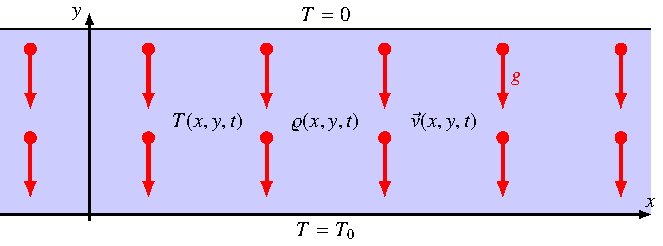
\includegraphics{chapters/2/lorenz-definition.pdf}
\caption{Definitionsgebiet für das Lorenz-Modell der Atmosphäre.
Gesucht sind Temperatur $T(x,y,t)$, Dichte $\varrho(x,y,t)$ und
Geschwindigkeit $\vec{v}(x,y,t)$ in einem Rechteckgebiet
$\mathbb R\times [0,\pi]$.
Die Temperatur ist an den Rändern vorgegeben, es gilt
$T(x,0,t)=T_0$ und $T(x,\pi,t)=0$.
Im Inneren Gebiet wird die Schwerkraft $g$ auf die Luft.
\label{skript:lorenzmodell definitionsgebiet}}
\end{figure}
Es soll ein dünner Schnitt durch die Atmosphäre modelliert werden.
Da die Atmosphäre im Vergleich zur Krümmung der Erdoberfläche sehr dünn ist,
können wir sie als eben annehmen.
Wir verwenden die Koordinate $x$ parallel zur Erdoberfläche und $y$ als Höhe
(Abbildung~\ref{skript:lorenzmodell definitionsgebiet}).
Gesucht ist also die Temperatur $T(x,y,t)$ und die Dichte $\varrho(x,y,t)$
in Abhängigkeit von Position und Zeit sowie der Geschwindigkeitsvektor
\[
\vec v
=
\begin{pmatrix}v_x\\v_y\end{pmatrix}
=
\begin{pmatrix}v_x(x,y,t)\\v_y(x,y,t)\end{pmatrix}.
\]
Die Funktionen $T$, $\varrho$, $v_x$ und $v_y$ sind definiert in einem
Streifen.
Der Einfachheit halber wählen wir die Höhe des Streifens als $\pi$.
Wir können dies erreichen, indem wir die Längeneinheit geeignet wählen:
ist $h$ die ``Dicke'' der Atmosphäre\footnote{Die Konvektion in der Atmosphäre,
welche vom Lorenz-Modell vor allem beschrieben wird, findet im Wesentlichen
nur im untersten Teil der Atmosphäre, der sogenannten Troposphäre statt.
Die Troposphäre zeichnet sich aus durch mehr oder weniger lineare
Temperaturabnahme bis zur Höhe der sogenannten Tropopause in etwa
10km Höhe.
Wir können also die Höhe der Tropopause als $h$ verwenden.}, wählen wir
$h/\pi$ als Längeneinheit.
Das Definitionsgebiet für die Funktionen ist daher $R=\mathbb R\times [0,\pi]$.

Die Temperatur der Atmosphäre an der Erdoberfläche wird im wesentlichen von
der Temperatur des Bodens bestimmt, der von der einfallenden Strahlung
erwärmt wird, es soll also $T(x,0,t)=T_0$ gelten.
Am oberen Rand des Schnittes schliesst die sehr dünne Hochatmosphäre an,
die im Wesentlichen in einem Strahlungsgleichgewicht mit der Umgebung steht.
Da wir die Dichte im wesentlichen als konstant ansehen wollen und damit
den Einfluss der Temperatur auf die Dichte nicht exakt modellieren wollen,
sind wir nicht gezwungen, eine bestimmte Temperaturskala zu verwenden.
Wir können daher willkürlich die Temperatur am oberen Rand als
$T(x,\pi,t)=0$ festlegen.

Auf das Medium im Streifen wirkt natürlich die Erdbeschleunigung,
die wir ebenfalls als konstant annehmen dürfen, da die Dicke der 
Atmosphäre im Vergleich zum Erdradius sehr klein ist.

\subsubsection{Stabile Atmosphäre}
\begin{figure}
\centering
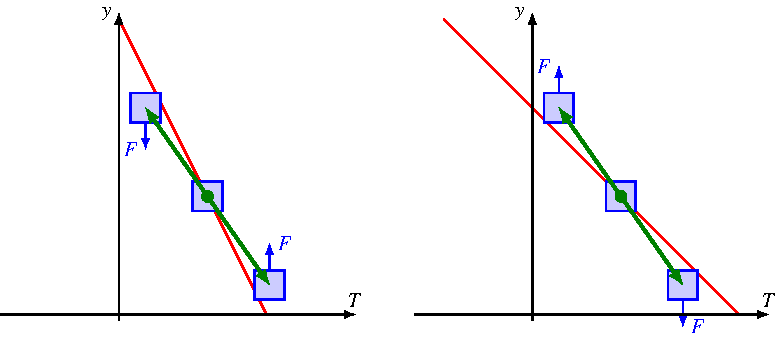
\includegraphics{chapters/2/lorenz-stabil.pdf}
\caption{Stabilität der Atmosphäre: bewegt sich ein Luftpaket in der
Atmosphäre nach oben oder unten, expandiert oder kontrahiert es und
verändert seine Temperatur adiabatisch (grün).
Ist diese Temperaturänderung grösser als der aktuelle Temperaturgradient
(links),
ändert sich die Dichte der Luft weniger stark als die der Umgebungsluft,
die Bewegung wird gestoppt, die Atmosphäre ist im Gleichgewicht.
Andernfalls wird die Bewegung beschleunigt, die Atmosphäre ist instabil
(rechts).
\label{skript:stabilitaet der atmosphaere}}
\end{figure}
Die Temperatur muss im Gebiet von unten nach oben abnehmen.
Aber auch der Druck muss mit zunehmender Höhe abnehmen. 
Wenn ein Luftpaket aufsteigt, wird es wegen des geringer werdenden
Druckes expandieren und damit adiabatisch abkühlen.
Wenn die Temperatur der umgebenden Luft schneller abnimmt als die
adiabatische Abkühlung, dann ist das Luftpaket in seiner neuen Höhe
wärmer und damit leichter als die Umgebung, es wird weiter ansteigen
(Abbildung~\ref{skript:stabilitaet der atmosphaere}).
Wenn die Temperatur der umgebenden Luft langsamer abnimmt als die
adiabatische Abkühlung, dann ist das Luftpaket in der neuen Höhe 
kälter und damit Dichter als die Umgebung, es wird wieder absinken.
Solange der Temperaturunterschied nicht zu gross ist, wird sich also ein
Zustand einstellen, in dem die Luft in Ruhe bleibt, der Wärmetransport
erfolgt ausschliesslich durch Wärmeleitung.

\subsubsection{Instabilität}
Bei genügend grosser Temperaturdifferenz wird die Atmosphäre jedoch
instabil, der Wärmetransport wird zusätzlich von Konvektion übernommen.
Die entstehenden Konvektionszellen können wegen der Translationssymmetrie
entlang der $x$-Achse an jeder beliebigen Stelle entstehen, es gibt also
unendlich viele Lösungen, von denen eine gewählt werden muss.
In der Realität würden kleine Temperaturfluktionen als Auslöser der 
Konvektion dienen.
Kleine Unterschiede in den Anfangsbedingungen führen also zu völlig
verschiedenen Strömungen.
% Abbildung?
Diese sensitive Abhängigkeit der Lösung von Anfangsbedingungen wird
oft als ein Kennzeichen von Chaos angesehen.
In Kapitel~\ref{chapter:lorenz} wird etwas vertieft auf die chaotischen
Aspekte des Lorenz-Systems eingegangen.

Im folgenden sollen zunächst die Gleichungen der Fluiddynamik auf die
vorliegende Situation spezialisiert werden.
Mit Hilfe eines geeigneten Ansatzes soll dann die partielle
Differentialgleichung weiter auf ein System von gewöhnlichen 
Differentialgleichungen reduziert werden.
In numerischen Simulationen soll schliesslich gezeigt werden, dass die 
Lorenz-Gleichungen tatsächlich chaotische Lösungen haben.

\subsubsection{Temperaturgleichung}
Wir haben in \eqref{skript:waermeleitungadvektion}
bereits eine Gleichung gefunden, welche den Wärmetransport in einem 
Fluid beschreibt.
Wir können daraus aber noch eine etwas einfacher zu handhabende Form
gewinnen, indem wir nur die Anomalie der Temperatur betrachten, also
\index{Anomalie}%
die Abweichung vom Temperaturprofil, welches sich bei einem ruhenden
Fluid einstellt. 
Aufgrund der gewählten Geometrie ist 
\[
T_0(x,y,t)= T_0\biggl(1- \frac{y}{\pi}\biggr)
\]
in einem ruhenden Fluid, wir setzen daher
\[
\vartheta(x,y,t)
= 
T(x,y,t)
-
T_0\biggl(1-\frac{y}{\pi}\biggr)
\qquad\text{oder}\qquad
T(x,y,t)
=
T_0\biggl(1-\frac{y}{\pi}\biggr)
+
\vartheta(x,y,t)
\]
und setzen dies in die Gleichung \eqref{skript:waermeleitungadvektion}
ein.
Wir erhalten
\begin{align*}
\frac{\partial\vartheta}{\partial t}
&=
\frac{\partial T}{\partial t}
&
\Delta T
&=
\Delta \vartheta
\\
-\vec{v}\cdot\nabla T
&=
-\vec{v}\cdot\nabla\vartheta
+v_y\frac{T_0}{\pi}.
\\
\Rightarrow
\qquad
\frac{\partial\vartheta}{\partial t}
&=
-\vec{v}\cdot\nabla \vartheta
+v_y\frac{T_0}{\pi}
+
\kappa\Delta \vartheta.
\end{align*}
Die Geschwindigkeit kann mit Hilfe von $\vec{v}=-\nabla \psi$ wieder
durch die Stromfunktion ausgedrückt werden.
\begin{equation}
\frac{\partial\vartheta}{\partial t}
=
-J\nabla\psi\cdot\nabla\vartheta
+\frac{T_0}{\pi}\frac{\partial\psi}{\partial x}
+\kappa\Delta\vartheta
=
\kappa\Delta\vartheta
+\frac{T_0}{\pi}\frac{\partial\psi}{\partial x}
-\frac{\partial \psi}{\partial y}\frac{\partial \vartheta}{\partial x}
+\frac{\partial \psi}{\partial x}\frac{\partial \vartheta}{\partial y}
=
\kappa\Delta\vartheta
+\frac{T_0}{\pi}\frac{\partial\psi}{\partial x}
-
\frac{\partial(\psi,\vartheta)}{\partial(x,y)}.
\label{skript:lorenzthetagl}
\end{equation}
Man beachte, dass die Gleichung bis auf den letzten Term linear 
in $\psi$ und $\vartheta$ ist.

\subsubsection{Bewegungsgleichung}
Die Bewegungsgleichung haben wir in
\eqref{skript:psidgl2}
bereits in die für ein zweidimensionales inkompressibles Fluid
geignete Form gebracht.
Da die Schwerkraft konstant ist, fällt der Terme $\nabla\times\vec{b}$
weg.

Aus der Boussinesq-Näherung
\eqref{skript:boussinesq}
erhalten wir noch einen Term, der den
Auftrieb beschreibt.
Auftrieb entsteht offenbar genau dann, wenn die Temperatur vom linearen
Temperaturprofil abweicht.
Wir nehmen an, dass die Dichteabweichung proportional zur Temperaturabweichung
ist, also
\[
\vec{b}
=
\begin{pmatrix}
0\\
-g(1-c\vartheta)
\end{pmatrix}
\qquad
\Rightarrow
\qquad
\nabla\times\vec{b}
=
c\frac{\partial\vartheta}{\partial x}
\]
mit der Proportionalitätskonstante $c$.
Damit erhalten wir die Bewegungsgleichung in der Form
\begin{equation}
\frac{\partial\Delta\psi}{\partial t}
=
\nu\Delta^2\psi 
+c\frac{\partial\vartheta}{\partial x}
-\frac{\partial(\psi,\Delta\psi)}{\partial(x,y)}.
\label{skript:lorenzpsigl}
\end{equation}
Man beachte, dass die Gleichung bis auf den letzten Term linear
in $\psi$ und $\vartheta$ ist.

\subsection{Grundgleichungen}
In den Gleichungen
\eqref{skript:lorenzthetagl}
und
\eqref{skript:lorenzpsigl}
haben wir ein partielles Differentialgleichungssystem für die beiden 
unbekannten Funktionen $\psi$ und $\vartheta$ gefunden, die wir
der besseren Übersicht halber nochmals als
\begin{equation}
\begin{aligned}
\frac{\partial\Delta\psi}{\partial t}
&=
\nu\Delta^2\psi 
+c\frac{\partial\vartheta}{\partial x}
-\frac{\partial(\psi,\Delta\psi)}{\partial(x,y)}
\\
\frac{\partial\vartheta}{\partial t}
&=
\kappa\Delta\vartheta
+\frac{T_0}{\pi}\frac{\partial\psi}{\partial x}
-
\frac{\partial(\psi,\vartheta)}{\partial(x,y)}
\end{aligned}
\label{skript:lorenzausgangsgleichung}
\end{equation}
hinschreiben.
Allerdings ist das System von dritter Ordnung, da erste Ableitungen von
$\psi$ und $\Delta\psi$ vorkommen.
Man sieht aber auch, dass keine anderen Ableitungen vorkommen als erste
Ableitungen von $\psi$ oder $\Delta\psi$.
Dies ist geeignet, die Diskussion zu vereinfachen, weshalb wird darauf
achten, diese Struktur nicht zu zerstören.

Wir können die linke Seite der Gleichungen zum Beispiel vektoriell schreiben
als
\[
\frac{\partial}{\partial t}
\begin{pmatrix}
\Delta\psi\\\vartheta
\end{pmatrix}
=
\frac{\partial}{\partial t}
\underbrace{
\begin{pmatrix}
\Delta &  0 \\
   0   &  1
\end{pmatrix}
}_{\displaystyle=D}
\underbrace{
\begin{pmatrix}
\psi\\\vartheta
\end{pmatrix}
}_{\displaystyle=u}
=
\frac{\partial}{\partial t} Du
\]
Entsprechend lassen sich die ersten zwei Terme auf der rechten Seite 
schreiben als
\[
\def\arraystretch{1.1}
\begin{pmatrix}
\nu\Delta^2     & \displaystyle c\frac{\partial}{\partial x}\\
\displaystyle \frac{T_0}{\pi}\frac{\partial}{\partial x}    &\kappa\Delta
\end{pmatrix}
\begin{pmatrix}
\psi\\\vartheta
\end{pmatrix}
=
Au.
\]
Die Operatoren $D$ und $A$ sind beide linear.

Für die Diskussion der Zeitentwicklung der Lösungen ist es nützlich,
die linearen Terme von den nichtlinearen zu trennen.
Wie bereits bemerkt treten Nichtlinearitäten nur in den
Funktionaldeterminanten auf.
Wir schreiben
\[
Nu
=
\def\arraystretch{1.9}
\begin{pmatrix}
\displaystyle
-\frac{\partial(\psi,\Delta\psi)}{\partial(x,y)}\\
\displaystyle
-\frac{\partial(\psi,\vartheta)}{\partial(x,y)}
\end{pmatrix}.
\]
Damit haben wir das Differentialgleichungssystem in der Form
\begin{equation}
\frac{\partial}{\partial t}Du
=
Au+Nu
\label{skript:allgemeinesmodell}
\end{equation}
mit den linearen Operatoren $D$ und $A$ und dem nichtlinearen Operator
$N$ schreiben.

Die allgemeine Form \eqref{skript:allgemeinesmodell} eines Klimamodells
ermöglicht uns, das Klimavorhersageproblem in dem etwas allgemeineren
Rahmen der Vorhersage für ein beliebiges nichtlineares dynamisches
System zu studieren.
Zwar ist \eqref{skript:allgemeinesmodell} immer noch ein partielles
Differentialgleichungssystem und die Operatororen $D$, $A$ und $N$
sind partielle Differentialoperatoren.
Wir können die in Abschnitt~\ref{section:pdeloesungen} zusammengestellten
Methoden anwenden um die Funktionen durch
Vektoren in einem endlichdimensionalen Vektorraum zu ersetzen, dann
werden $D$ und $A$ zu linearen Abbildungen, die durch Matrizen beschrieben
werden können, und $N$ wird zu einer nichtlinearen Funktion auf einem
endlichdimensionalen Vektorraum.
Das Klimamodell wird also zu einer nichtlinearen gewöhnlichen
Differentialgleichung in einem endlichdimensionalen Raum.
Solche Differentialgleichungen sind im Detail studiert worden und ihre
Eigenschaften sind sehr gut verstanden.
In Kapitel~\ref{chapter:dgl} werden wir einen Teil der gut ausgebauten
Theorie zusammenfassen.
Den Weg von \eqref{skript:allgemeinesmodell} zu einer gewöhnlichen
Differentialgleichung in nur drei Dimensionen soll im folgenden 
Abschnitt~\ref{subsection:umwandlung} vorgeführt werden.

% XXX Diskussion des unendlichdimensionalen dynamischen Systems

\subsection{Umwandlung in ein gewöhnliches Differentialgleichungssystem\label{subsection:umwandlung}}
\begin{figure}
\centering
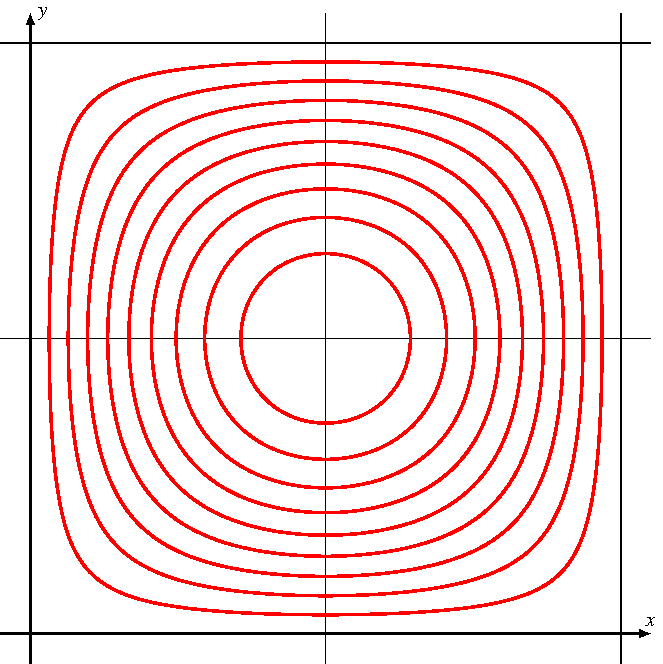
\includegraphics{chapters/2/konvektion.pdf}
\caption{Stromlinien in einer einzelnen Konvektionszelle
\label{skript:stromlinien konvektion}}
\end{figure}
Ausgehend von
\eqref{skript:lorenzausgangsgleichung}
versuchen wir nun, eine gewöhnliche Differentialgleichung zu gewinnen,
welche näherungsweise wiedergibt, was passiert, wenn im betrachteten
System Konvektion einsetzt.
Eine einzelne Konvektionszelle hat Stromlinien, wie sie in Abbildung
\ref{skript:stromlinien konvektion}
dargestellt sind.
Vernachlässigt man in der ersten der Differentialgleichungen
\eqref{skript:lorenzausgangsgleichung}
$\vartheta$ und den nichtlinearen Term, bleibt eine Wärmeleitungsgleichung
für $\Delta \psi$.
\subsubsection{Separationsansatz}
Die Wärmeleitungsgleichung auf einem Rechteckgebiet 
einer solchen Zelle könnte man mit einem Separationsansatz zu lösen
versuchen, dies würde auf Lösungen der Form
$\sin(ax)\sin(y)$
führen.
Wir versuchen daher eine Lösung für $\psi(x,y,t)$ in der etwas
allgemeineren Form
\begin{equation}
\psi(x,y,t)
=
X(t) \sin(ax)\sin(y)
\label{skript:psiansatz}
\end{equation}
zu finden.
Die Konvektion sorgt dafür, dass im Bereich grosser
Strömungsgeschwindigkeit der Temperaturgradient stark vom linearen Verlauf
abweicht.
Die vertikale Strömungsgeschwindigkeit ist bei $0$ und $\pi$ hoch, also
dort wo $\cos(ax)$ gross ist.
Wir setzen daher die Lösung für die Temperatur $\vartheta(x,y,t)$ an in der
Form
\begin{equation}
\vartheta(x,y,t)
=
Y(t) \cos(ax) \sin(y) - Z(t) \sin(2y).
\label{skript:thetaansatz}
\end{equation}
Das Ziel ist, für die drei Funktionen $X(t)$, $Y(t)$ und $Z(t)$
gewöhnliche Differentialgleichungen aufzustellen, also die Ortsabhängigkeit
der Lösungsfunktionen vollständig zu eliminieren.

\subsubsection{Ableitungen}
Wir können allerdings nicht erwarten, dass dies exakte Lösungen sind.
Beim Einsetzen in die Differentialgleichungen werden auch noch
andere Terme entstehen.
Unter der Annahme, dass die genannten Terme die Gestalt der Stromlinien
genau genug wiederzugeben in der Lage sind, vernachlässigen wir alle
Terme, die sich nicht als Vielfache der Funktionen
\begin{equation}
\sin(ax)\sin(y),
\qquad
\cos(ax)\sin(y)
\qquad\text{und}\qquad
\sin(2y)
\label{skript:funktionsauswahl}
\end{equation}
schreiben lassen.

Wir müssen jetzt also die Lösungsansätze
\eqref{skript:psiansatz}
und
\eqref{skript:thetaansatz}
in die Differentialgleichungen
\eqref{skript:lorenzausgangsgleichungen}
einsetzen.
Die linke Seite ist jeweils einfach, da die Zeitabhängigkeit nur noch
in den Funktion $X(t)$, $Y(t)$ und $Z(t)$ steckt.
Auf der linken Seite können wir daher einfach $X(t)$ durch $\dot X(t)$
ersetzen und analog für die anderen beiden Koeffizientenfunktionen.

Die Ortsableitungen geben etwas mehr zu tun:
\begin{align*}
\frac{\partial}{\partial x}\psi
&=
X(t)a\cos(ax)\sin(y)
&
\frac{\partial}{\partial y}\psi
&=
X(t)\sin(ax)\cos(y)
\\
\frac{\partial^2}{\partial x^2}\psi
&=
-X(t)a^2\sin(ax)\sin(y)
&
\frac{\partial^2}{\partial y^2}\psi
&=
-X(t)\sin(ax)\sin(y)
\\
\Delta\psi
&=-(a^2+1)\psi
&
\Delta^2 \psi
&=
(a^2+1)^2\psi.
\end{align*}
für $\psi$ und
\begin{align*}
\frac{\partial}{\partial x}\vartheta
&=
-aY(t) \sin(ax) \sin(y)
&
\frac{\partial}{\partial y}\vartheta
&=
Y(t) \cos(ax) \cos(y) - 2 Z(t)\cos(2y)
\\
\frac{\partial^2}{\partial x^2}\vartheta
&=
-a^2Y(t) \cos(ax) \sin(y)
&
\frac{\partial^2}{\partial y^2}\vartheta
&=
-Y(t) \cos(ax) \sin(y)
+4Z(t)\sin(2y)
\\
\Delta\vartheta
&=\mathrlap{-(a^2+1)Y(t)\cos(ax)\sin(y)+4Z(t)\sin(2y)}
\end{align*}
für $\vartheta$.
In den Differentialgleichungen brauchen wir aber noch die
Funktionaldeterminanten für die nichtlinearen Terme:
\begin{align*}
\frac{\partial(\psi,\Delta\psi)}{\partial(x,y)}
&=
\frac{\partial\psi}{\partial x} \frac{\partial\Delta\psi}{\partial y}
-
\frac{\partial\psi}{\partial y} \frac{\partial\Delta\psi}{\partial x}
=
-(a^2+1)\biggl(
\frac{\partial\psi}{\partial x} \frac{\partial\psi}{\partial y}
-
\frac{\partial\psi}{\partial y} \frac{\partial\psi}{\partial x}
\biggr)
=0
\\
\frac{\partial(\psi,\vartheta)}{\partial(x,y)}
&=
\frac{\partial\psi}{\partial x} \frac{\partial\vartheta}{\partial y}
-
\frac{\partial\psi}{\partial y} \frac{\partial\vartheta}{\partial x}
\\
&=
X(t)\biggl(
a \cos(ax)\sin(y)
\bigl(Y(t) \cos(ax) \cos(y) - 2Z(t)\cos(2y)\bigr)
\\
&\qquad
-
\sin(ax)\cos(y)
\bigl(-aY(t) \sin(ax) \sin(y) \bigr)
\biggr)
\\
&=
X(t)(a(\underbrace{\cos^2(ax)+\sin^2(ax)}_{\displaystyle=1})
Y(t)\underbrace{\sin(y)\cos(y)}_{\displaystyle{\textstyle\frac12}\sin(2y)}-2a\cos(ax)\sin(y)Z(t)\cos(2y))
\\
&=
\frac12aX(t)Y(t) \sin(2y)
-
2a X(t)Z(t) \cos(ax)\sin(y)\cos(2y)
\\
&=
\frac12aX(t)Y(t) \sin(2y)
-
2a X(t)Z(t) \cos(ax)\frac12(\sin(-y)+\sin(3y))
\\
&=
\frac12aX(t)Y(t) \sin(2y)
+
2aX(t)Z(t) \cos(ax)\sin(y)
-
2aX(t)Z(t) \cos(ax)\sin(3y).
\end{align*}
\subsubsection{Approximation}
Der letzte Term kann nicht durch Funktionen aus der Liste
\eqref{skript:funktionsauswahl}
ausgedrückt werden, und muss daher vernachlässigt werden.
Setzen wir jetzt diese Ableitungen in die Differentialgleichungen
ein, erhalten wir
\begin{align*}
-(a^2+1)
\dot X(t) \sin(ax)\sin(y)
&=
\nu (a^2+1)^2 X(t)\sin(ax)\sin(y)
-acY(t)\sin(ax)\sin(y)
\\
\dot Y(t)\cos(ax)\sin(y)-\dot Z(t)\sin(2y)
&=
-\kappa (a^2+1)Y(t)\cos(ax)\sin(y) +4\kappa Z(t)\sin(2y)
\\
&\qquad +\frac{T_0}{\pi} X(t)a\cos(ax)\sin(y)
\\
&\qquad
-\frac{a}2X(t)Y(t)\sin(2y) - 2aX(t)Z(t)\cos(ax)\sin(y).
\end{align*}
\subsubsection{Gewöhnliche Differentialgleichungen}
Wir vergleichen die Koeffizienten der Funktionen aus der Liste
\eqref{skript:funktionsauswahl}
dann erhalten wir das Differentialgleichungssystem 

%(%i26)                               dglX
%             2       d                           4      2
%(%o26)   (- a  - 1) (-- (X(t))) + a c Y(t) + (- a  - 2 a  - 1) nu X(t)
%                     dt
%(%i27)                               dglY
%         a X(t) T_0   d                          2
%(%o27) - ---------- + -- (Y(t)) + a X(t) Z(t) + a  kappa Y(t) + kappa Y(t)
%            %pi       dt
%(%i28)                               dglZ
%                     d                          a X(t) Y(t)
%(%o28)             - -- (Z(t)) - 4 kappa Z(t) + -----------
%                     dt                              2
\begin{equation}
\begin{aligned}
\dot X(t)
&=
-\nu(a^2+1)X(t)
+\frac{ac}{a^2+1}Y(t)
\\
\dot Y(t)
&=
\frac{aT_0}{\pi}X(t)
-(a^2+1)\kappa Y(t)
-aX(t)Z(t)
\\
\dot Z(t)
&=
-4\kappa Z(t)
+\frac{a}{2}X(t)Y(t)
\end{aligned}
\label{skript:lorenz:dim}
\end{equation}
für die Koeffizientenfunktionen $X(t)$, $Y(t)$ und $Z(t)$.

\subsection{Dimensionslose Schreibweise}
Die Form \eqref{skript:lorenz:dim} der Lorenz-Gleichungen ist für eine
Diskussion der Lösungen nicht besonders gut geeignet.
Die komplizierte Form der Koeffizienten erschwert den Überblick.
Ein übersichtlicheres System erhält man, wenn man die folgenden
Ersetzungen vornimmt:
\begin{align*}
x
&=
\frac{a}{\kappa(a^2+1)\sqrt{2}}
\,
X,
\\
y
&=
\frac{a^2 c}{\kappa \nu (a^2+1)\sqrt{2}}
\,
Y,
\\
z
&=
\frac{a^2c}{\kappa\nu(a^2+1)^3}
\,
Z,\qquad\text{und}
\\
t'
&=
\kappa (a^2+1)\, t.
\end{align*}
Damit werden die Differentialgleichungen zu
\begin{align*}
\dot x &= -\sigma x + \sigma y\\
\dot y &= \varrho x - y - x z\\
\dot z &= -\beta z + x y
\end{align*}
mit den Konstanten
\begin{align*}
\sigma
&=
\frac{\nu}{\kappa},
&
\varrho
&=
\frac{a^2cT_0}{\kappa\nu\pi(a^2+1)^3},
&&\text{und}&
\beta
&=
\frac{4}{a^2 +1}.
\end{align*}
Es stellt sich heraus, dass gewisse Lösungen dieser Differentialgleichung
chaotisches Verhalten zeigen.
Damit sind der Verhersagbarkeit von Wetterphänomenen bereits prinzipielle
Grenzen gesetzt.
Dies besagt aber nicht, dass sich das Klima nicht vorhersagen lässt,
sondern nur, dass das Lorenzmodell nicht dazu geeignet ist, den
Wärmetransport durch Konvektion in der Atmosphäre über längere Zeit
zu modellieren.
Die in Kapitel~\ref{chapter:zonenmodelle} dargestellten Modelle sind
dazu durchaus in der Lage.






